
Product line engineering is a very common practice in the manufacturing industry. It allows the \textit{large-scale production of goods and services tailored to individual customers' needs}, called \emph{mass customisation} \cite{Pohl2005}. Success stories come from the automotive industry where product line have been invented in the first half of the 20th century. Under the market pressure, the development of product line engineering allows nowadays a customer to configure his car and have it delivered within three months. Product line and mass customisation are also used in other domains to personalise services for instance: with the latest developments of medical research (\eg imaging, DNA analysis, \etc) treatments plans are now customised to target the exact disease, reduce side effects, and accelerate recovery. To be tractable, a product line relies on \emph{platforms}, \ie \textit{any base of technologies on which other technologies or processes are built} \cite{Pohl2005}.

\glsreset{SPL}

\gls{SPL} engineering is the application of those ideas to software development: it is \textit{the paradigm to develop software applications using platforms and mass customisation} \cite{Pohl2005}. One software, \ie a \emph{product}, is built by combining \emph{commonalities}, common to all the products of the product line, and \emph{variabilities}, specific to only some products. 

This chapter presents the main ideas and concepts of \gls{SPL} engineering used in this thesis. Section \ref{sec:sple} presents the development of \glspl{SPL} and section \ref{sec:features} presents how variability is captured and managed in this process. Section \ref{sec:splbehaviouralmodeling} discusses different modelisation approaches to describe \gls{SPL} behaviour, including featured transition systems, the formalism we use in the remainder of this thesis.


%%%%%%%%%%%%%%%%%%%%%%%%%%%%%%%%%%%%%%%%%%%%%%%%%%
\section{Software product line engineering}
%%%%%%%%%%%%%%%%%%%%%%%%%%%%%%%%%%%%%%%%%%%%%%%%%%

\label{sec:sple}

\begin{figure}
	\centering
	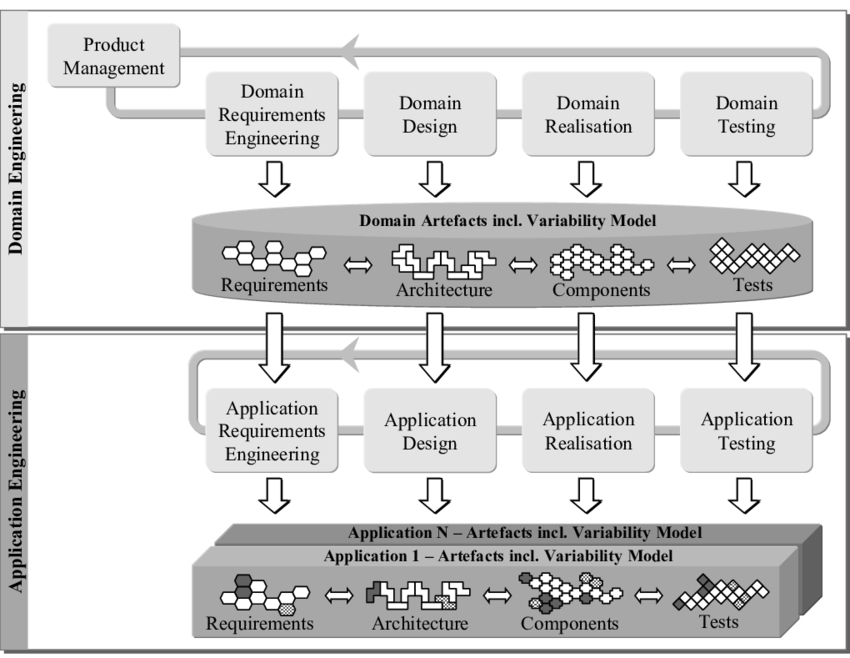
\includegraphics[width=110mm]{spldev-pohl}
	\caption{The \gls{SPL} development processes \cite{Pohl2005}}
	\label{fig:spldev}
\end{figure}

\gls{SPL} engineering consists in two development processes presented in Figure \ref{fig:spldev} \cite{Pohl2005}: \emph{domain engineering}, where \textit{commonalities and variabilities of the product line are defined and realised}, and \emph{application engineering}, where \textit{applications of the product line are built by reusing domain artefacts and exploiting the product line variability}. Each one of those two processes consists of several activities (including testing) and produces different artefacts. Domain artefacts are reused during application engineering in order to built one particular product. 

This thesis focuses on behavioural testing at the domain level. We seek to select \emph{relevant behaviours}, as well as \emph{relevant products} able to execute those behaviours in order to ensure that the \gls{SPL} fulfils its specification. To do so, we use a \emph{model-based} approach, with a model abstracting the behaviour of all the \gls{SPL} (including product-specific and SPL-common behaviours).

Commonalities and variabilities are captured trough the notion of \emph{feature}. A feature is a \textit{characteristic or end-user-visible behaviour of a software system} \cite{Apel2013}. It is a first-class abstraction that helps to reason about the \gls{SPL} \cite{Classen2008}. In practice, features are mapped to domain artefacts (or parts of domain artefacts) that are combined to form products. The derivation of one product consists in selecting a valid set of features, called \emph{configuration}, with the intended characteristics of the product, and combining the domain artefacts linked to those features. All the valid combinations of features are described in a \emph{feature model}.


%%%%%%%%%%%%%%%%%%%%%%%%%%%%%%%%%%%%%%%%%%%%%%%%%%
\section{Feature models}
%%%%%%%%%%%%%%%%%%%%%%%%%%%%%%%%%%%%%%%%%%%%%%%%%%

\label{sec:features}

\glsreset{FM}

\glspl{FM} describe all the valid combinations of features for \glspl{SPL}. They have been introduced by Kang \etal in the \gls{FODA} method \cite{Kang1990} using a graphical representation. Lot of other graphical \cite{Antkiewicz2004,Trinidad2008,Beuche2013,Leich2005} and textual \cite{Mendonca2009,Classen2011a} representations have been proposed and formalised \cite{Schobbens2007,Batory2005} since. In this thesis, we focus on graphical boolean \glspl{FM} and their equivalence in \gls{TVL} \cite{Classen2011a}. 

\begin{figure}
	\centering
	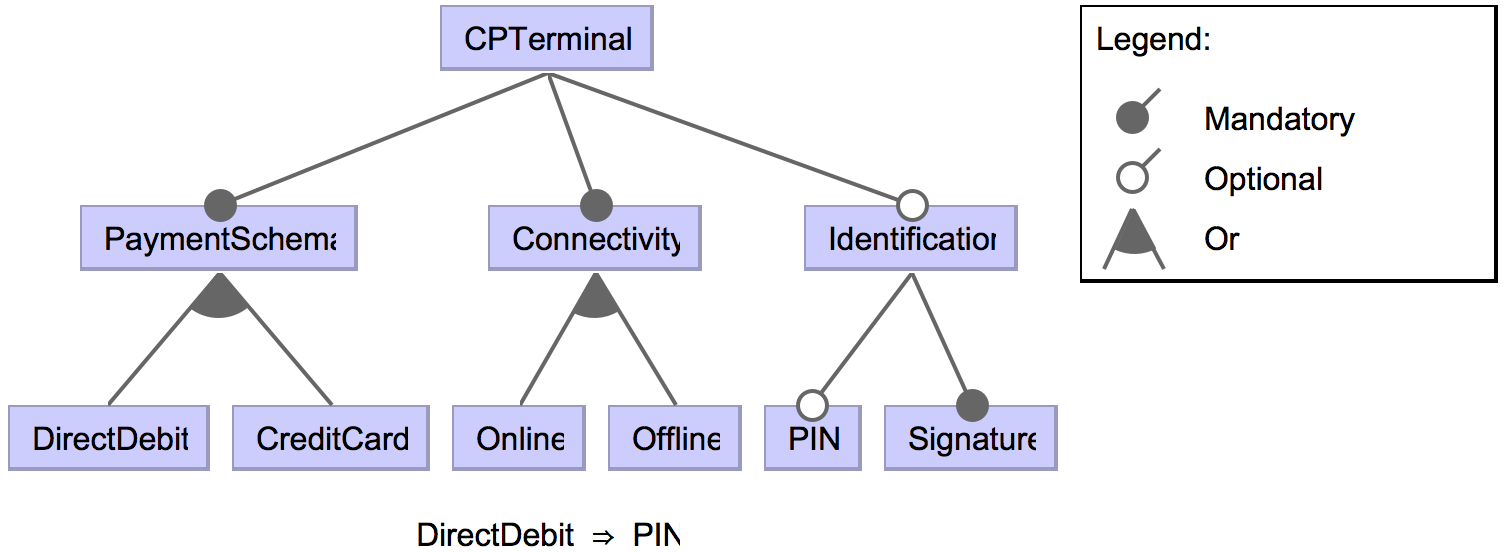
\includegraphics[width=100mm]{cpterminal-simplified-fm}
	\caption{Card payment terminal simplified feature model}
	\label{fig:cpterminalsimplifiedfm}
\end{figure}

A \gls{feature model} is organised in a tree-like structure (formally a directed acyclic graph). The root feature, always present in all products, is decomposed in sub-features using \textit{and} (all sub-features are selected if the parent feature is selected), \textit{or} (at-least one sub-feature is selected if the parent feature is selected), and \textit{xor} (exactly one sub-feature is selected if the parent feature is selected) relations. For instance, Figure \ref{fig:cpterminalsimplifiedfm} presents a (simplified) feature model for a card payment terminal product line. Root feature (\textit{CPTerminal}) is decomposed into two mandatory features (\textit{Pay\-ment\-Sche\-ma} and \textit{Con\-necti\-vi\-ty}) and one optional feature (\textit{Iden\-ti\-fica\-tion}). \textit{Pay\-ment\-Sche\-ma} (specifying if the terminal supports credit or debit cards) and \textit{Con\-necti\-vi\-ty} (specifying if the terminal is connected or not) features are decomposed into sub-features using a \textit{or} relation. Additionally, feature models may have cross-tree constraints expressed as boolean expressions over the features, \eg  \textit{Di\-rect\-De\-bit} $\Rightarrow$ \textit{PIN}, specifying that debit card payment requires PIN authentication.

\begin{lstlisting}[language=TVL,
float,
label=lst:cpterminalsimplifiedtvl,
caption={Card payment terminal simplified feature model in TVL format}]
root CPTerminal {
	group allOf {
		PaymentSchema,
		Connectivity,
		opt Identification
	}
} 

PaymentSchema {
	group someOf {
		DirectDebit,
		CreditCard
	}
	DirectDebit -> PIN; (*@\label{lst:cpterminalsimplifiedtvl:line:constraint}@*)
} 

Connectivity group someOf {
	Online,
	Offline
}

Identification group allof {
	opt PIN,
	Signature
}
\end{lstlisting}

Listing \ref{lst:cpterminalsimplifiedtvl} presents the TVL version of Figure \ref{fig:cpterminalsimplifiedfm}. In this case, features are decomposed in sub-features using \texttt{allOf} (\textit{and}), \texttt{someOf} (\textit{or}), or \texttt{oneOf} (\textit{xor}) relations. Additional cross-tree constraints (on line \ref{lst:cpterminalsimplifiedtvl:line:constraint}) may be specified and optional features are indicated using \texttt{opt} keyword.

The semantics of a feature model $d$, denoted $\Sem{d}$, corresponds to all the valid products allowed by the feature model. In the remainder of this thesis, we consider only \emph{boolean feature models}, \ie feature models where features have boolean values: \textit{true} if the feature is selected and \textit{false} otherwise. Since a boolean feature model may be transformed into a \gls{CNF} formula \cite{Batory2005}, denoted $\CNF(d)$, its semantics corresponds to all the feature assignments that satisfies this formula. This may be computed using \gls{SAT} or \gls{BDD} solvers \cite{Liang2015,Mendonca2008}.


%%%%%%%%%%%%%%%%%%%%%%%%%%%%%%%%%%%%%%%%%%%%%%%%%%%%%%%%%%%%%
\section{Behavioural modellisations of software product lines}
%%%%%%%%%%%%%%%%%%%%%%%%%%%%%%%%%%%%%%%%%%%%%%%%%%%%%%%%%%%%%

\label{sec:splbehaviouralmodeling}

Modern software systems are complex to build and maintain, counting thousands of lines of codes to achieve various purposes under different kinds of constraints (\eg time response, security, availability, \etc). To manage this complexity, software engineers use modeling \cite{swebok2014}. This allows to abstract the system by focusing on some of its aspects. For instance, feature models focus on the features of a product line and their constraints. In \gls{SPL} engineering, complexity worsen due to the variability inherent to product line. Models have to take features into account to represent this variability.

This section presents different modelling approaches to represent the behaviour of a software product line. Those approaches may be decomposed into two categories \cite{Apel2013}: \emph{annotation}-based approaches and \emph{composition}-based approaches. Annotation-based approaches annotate a common model to indicate which parts of the model belongs to which feature(s). During product derivation (\ie selection of the features of a product), parts of the model marked with unselected features are removed to give a model of the product. Composition-based approaches models features as a set of composable model parts. During product derivation, those parts are combined to form the model of the product. 

%----------------------------------------------------
\subsection{Composition-based modelling approaches}
%----------------------------------------------------

\begin{figure}[t]
	\centering
	\subbottom[Base model]{
		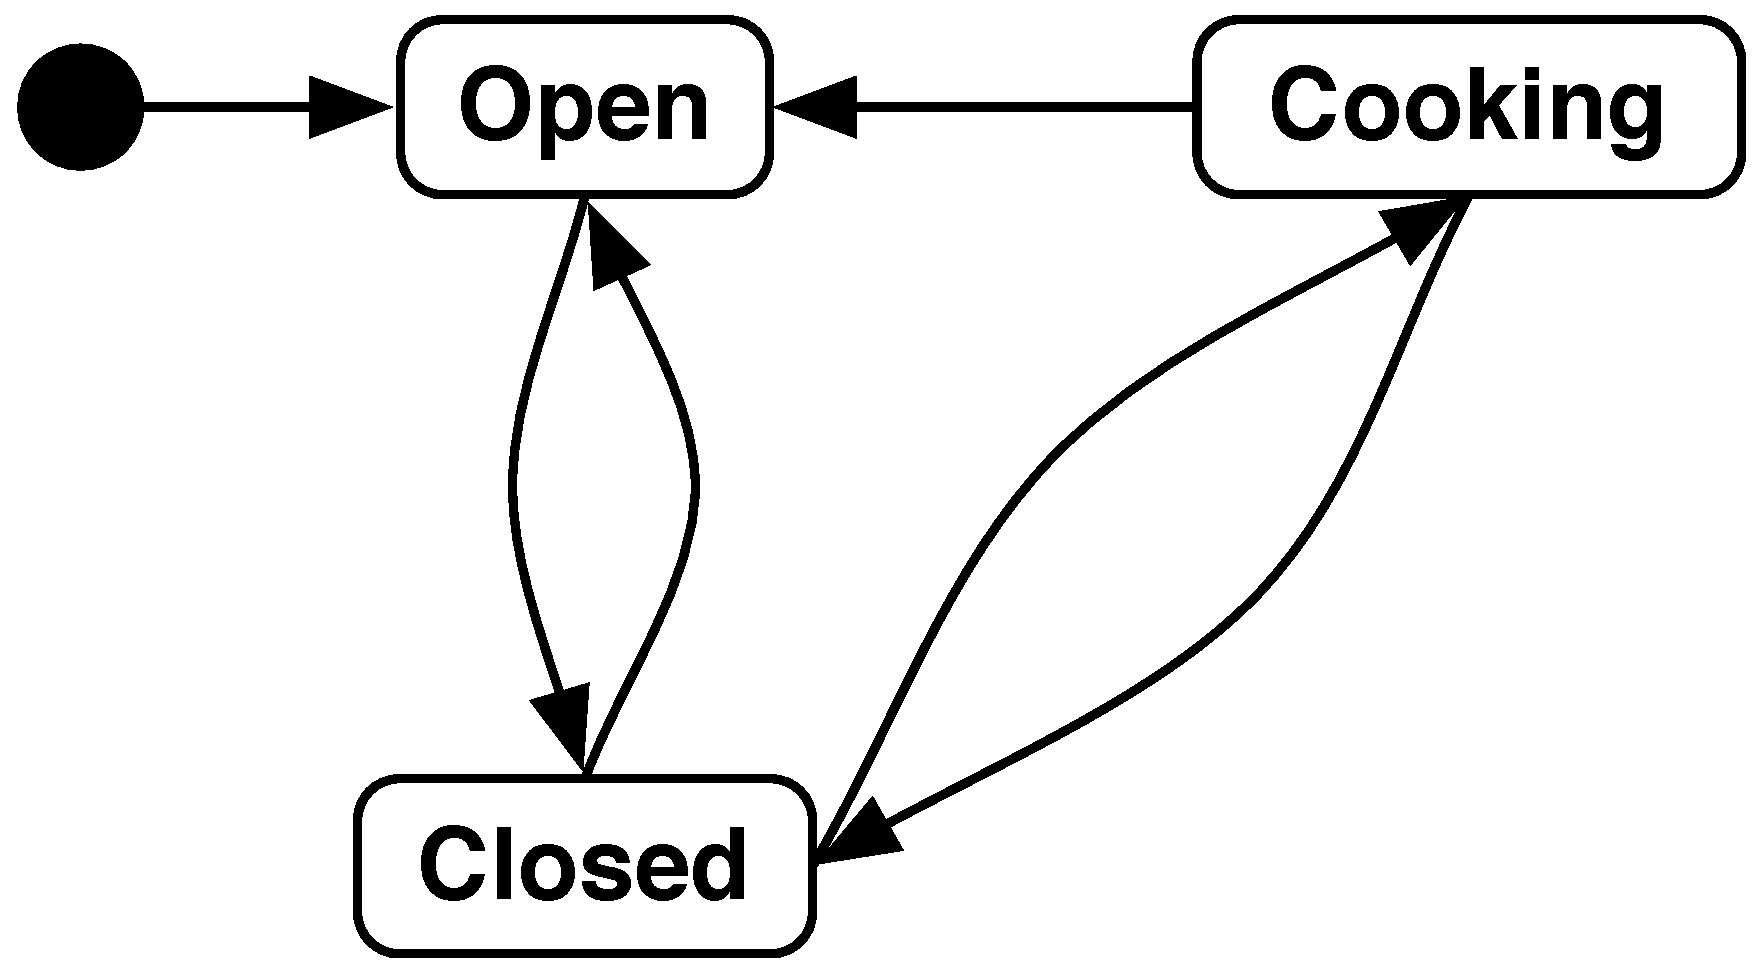
\includegraphics[width=38mm]{aom-base}
		\label{fig:aombase}
	}	
	\subbottom[Feature aspect]{
		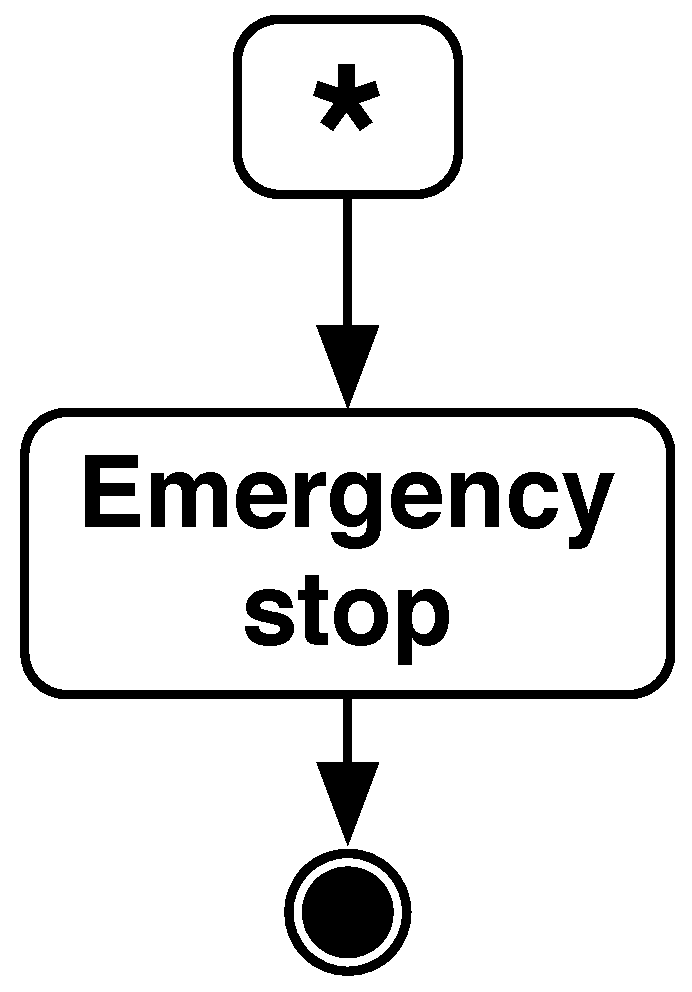
\includegraphics[width=14mm]{aom-aspect}
		\label{fig:aomaspect}
	}	
	\subbottom[Product model]{
		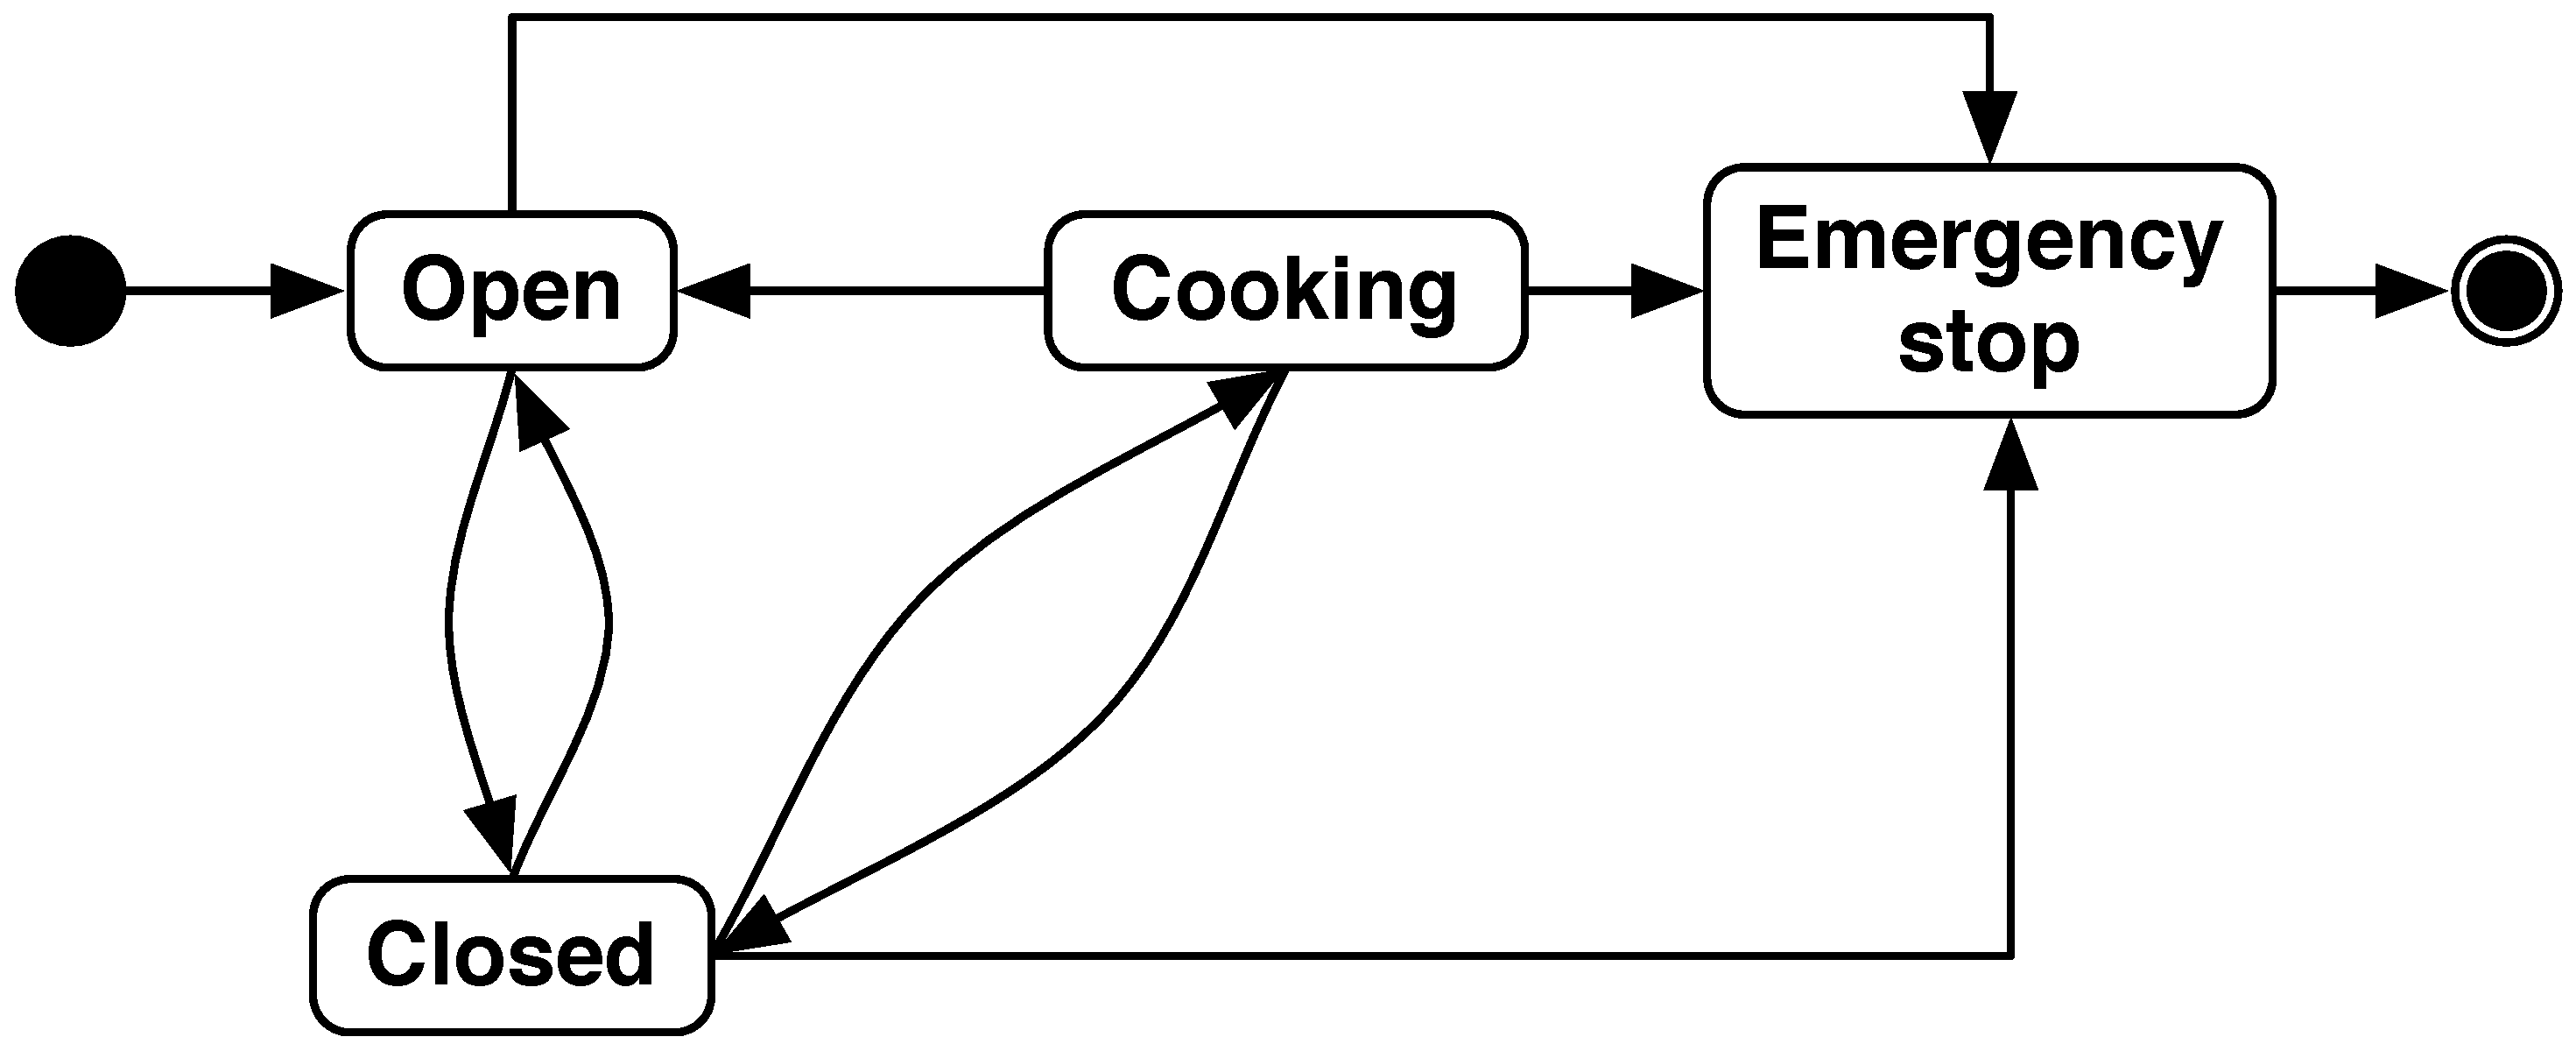
\includegraphics[width=54mm]{aom-result}
		\label{fig:aomresult}
	}
	\caption{\gls{SPL} behavioural composition-based modelling example \cite{Rashid2011}}
\end{figure}

Most composition-based modelling approaches are based on \emph{aspect oriented modelling} \cite{Rashid2011,Groher2009}. A base model representing the behaviour common to al the products of the product line is modified by weaving aspects specific to one or more features. For instance, Figure \ref{fig:aombase} presents the state machine base model of a oven in a smart home \cite{Rashid2011}. When a product with the feature \textit{emergency stop} is derived, the aspect from Figure \ref{fig:aomaspect} is weaved in the base model to give the state machine of the product in Figure \ref{fig:aomresult}. To decide where to be applied, the aspect must specify one or more pointcuts using a pointcut expression: '\texttt{*}' in Figure \ref{fig:aomaspect}.

Various formalisms based on transition systems \cite{Asirelli2012,Li2002,Li2002a,Li2005,Krishnamurthi2004,Fisler2001,Cordy2012} and Input-Output automata \cite{Lauenroth2009,Lauenroth2010} exist. Other composition-based modelling approaches are extensions of existing modelling languages where feature aspects may be weaved at some specific points of the system \cite{Altisen2006,Apel2010,Batory2008,Calder2006,Gondal2011,Schaefer2010,Millo2012a,Nelson2001,Poppleton2007,Sorge2009}. Finally, UML models like state machines \cite{Shaker2012,Shaker2012a} and sequence diagrams \cite{Greenyer2012} have been extended to support composition-based modelling.


%----------------------------------------------------
\subsection{Annotation-based modelling approaches}
%----------------------------------------------------

There exists several annotation-based modelling approaches to represent the behaviour of a software product line. Most of them consider a based model annotated with variability information indicating which products of the product line it belongs to. State-based models include for instance Petri nets \cite{Muschevici2010,Puschel2012,Heuer2013}, modal I/O automata \cite{Larsen2007}, \glspl{MTS} \cite{Asirelli2011,Asirelli2011a,Asirelli2011b,Fantechi2008,Fischbein2006,TerBeek2013,terBeek2011}, \glspl{FTS} \cite{Classen2011-thesis,Classen2013b,Classen2011,Classen2010}, and finite state machines \cite{Sabouri2012,Sabouri2012}. Other formalisms include PL-CSS  (a process algebra) \cite{Gruler2008} and higher-level formalisms like UML activity diagrams \cite{Heuer2013}. 

\glsreset{LTS}

Researches on annotation-based models for software product line verification have been conducted for years and are still developed by the model-checking community. Amongst all the existing notations, in this thesis, we focus on those derived from \gls{LTS}, a simple and yet expressive formalism to model the behaviour of a system:
%
\begin{definition}[\acrfull{LTS} \cite{Baier2008}] \label{def:ts}
A LTS is a tuple $(S,$ $\Act,$ $\trans,$ $i)$, where:
\begin{itemize}
\item $S$ is a set of \emph{states};
\item $\Act$ is a set of \emph{actions};
\item $\trans \ \subseteq S \times \Act \times S$ is a \emph{transition} relation (with $(s_1, \alpha, s_2) \in \trans$, denoted $s_1 \overset{\alpha}{\longrightarrow} s_2$);
\item and $i \in S$ is the \emph{initial state}.
\end{itemize}
\end{definition} 
%
This choice is motivated by the existence of powerful modelling languages \cite{Asirelli2011a,Fantechi2008,TerBeek2013}, algorithms \cite{Classen2010,Classen2013b}, and tools \cite{Asirelli2011b,Cordy2013} developed by the model-checking community. Also, lot of other higher-level formalisms may be translated to \gls{LTS} \cite{Devroey2015c} allowing to make our results easily applicable to other modelling  languages.

%-------------------------------------------
\subsection{Featured transition system}
%-------------------------------------------

\begin{figure}[t]
	\centering
	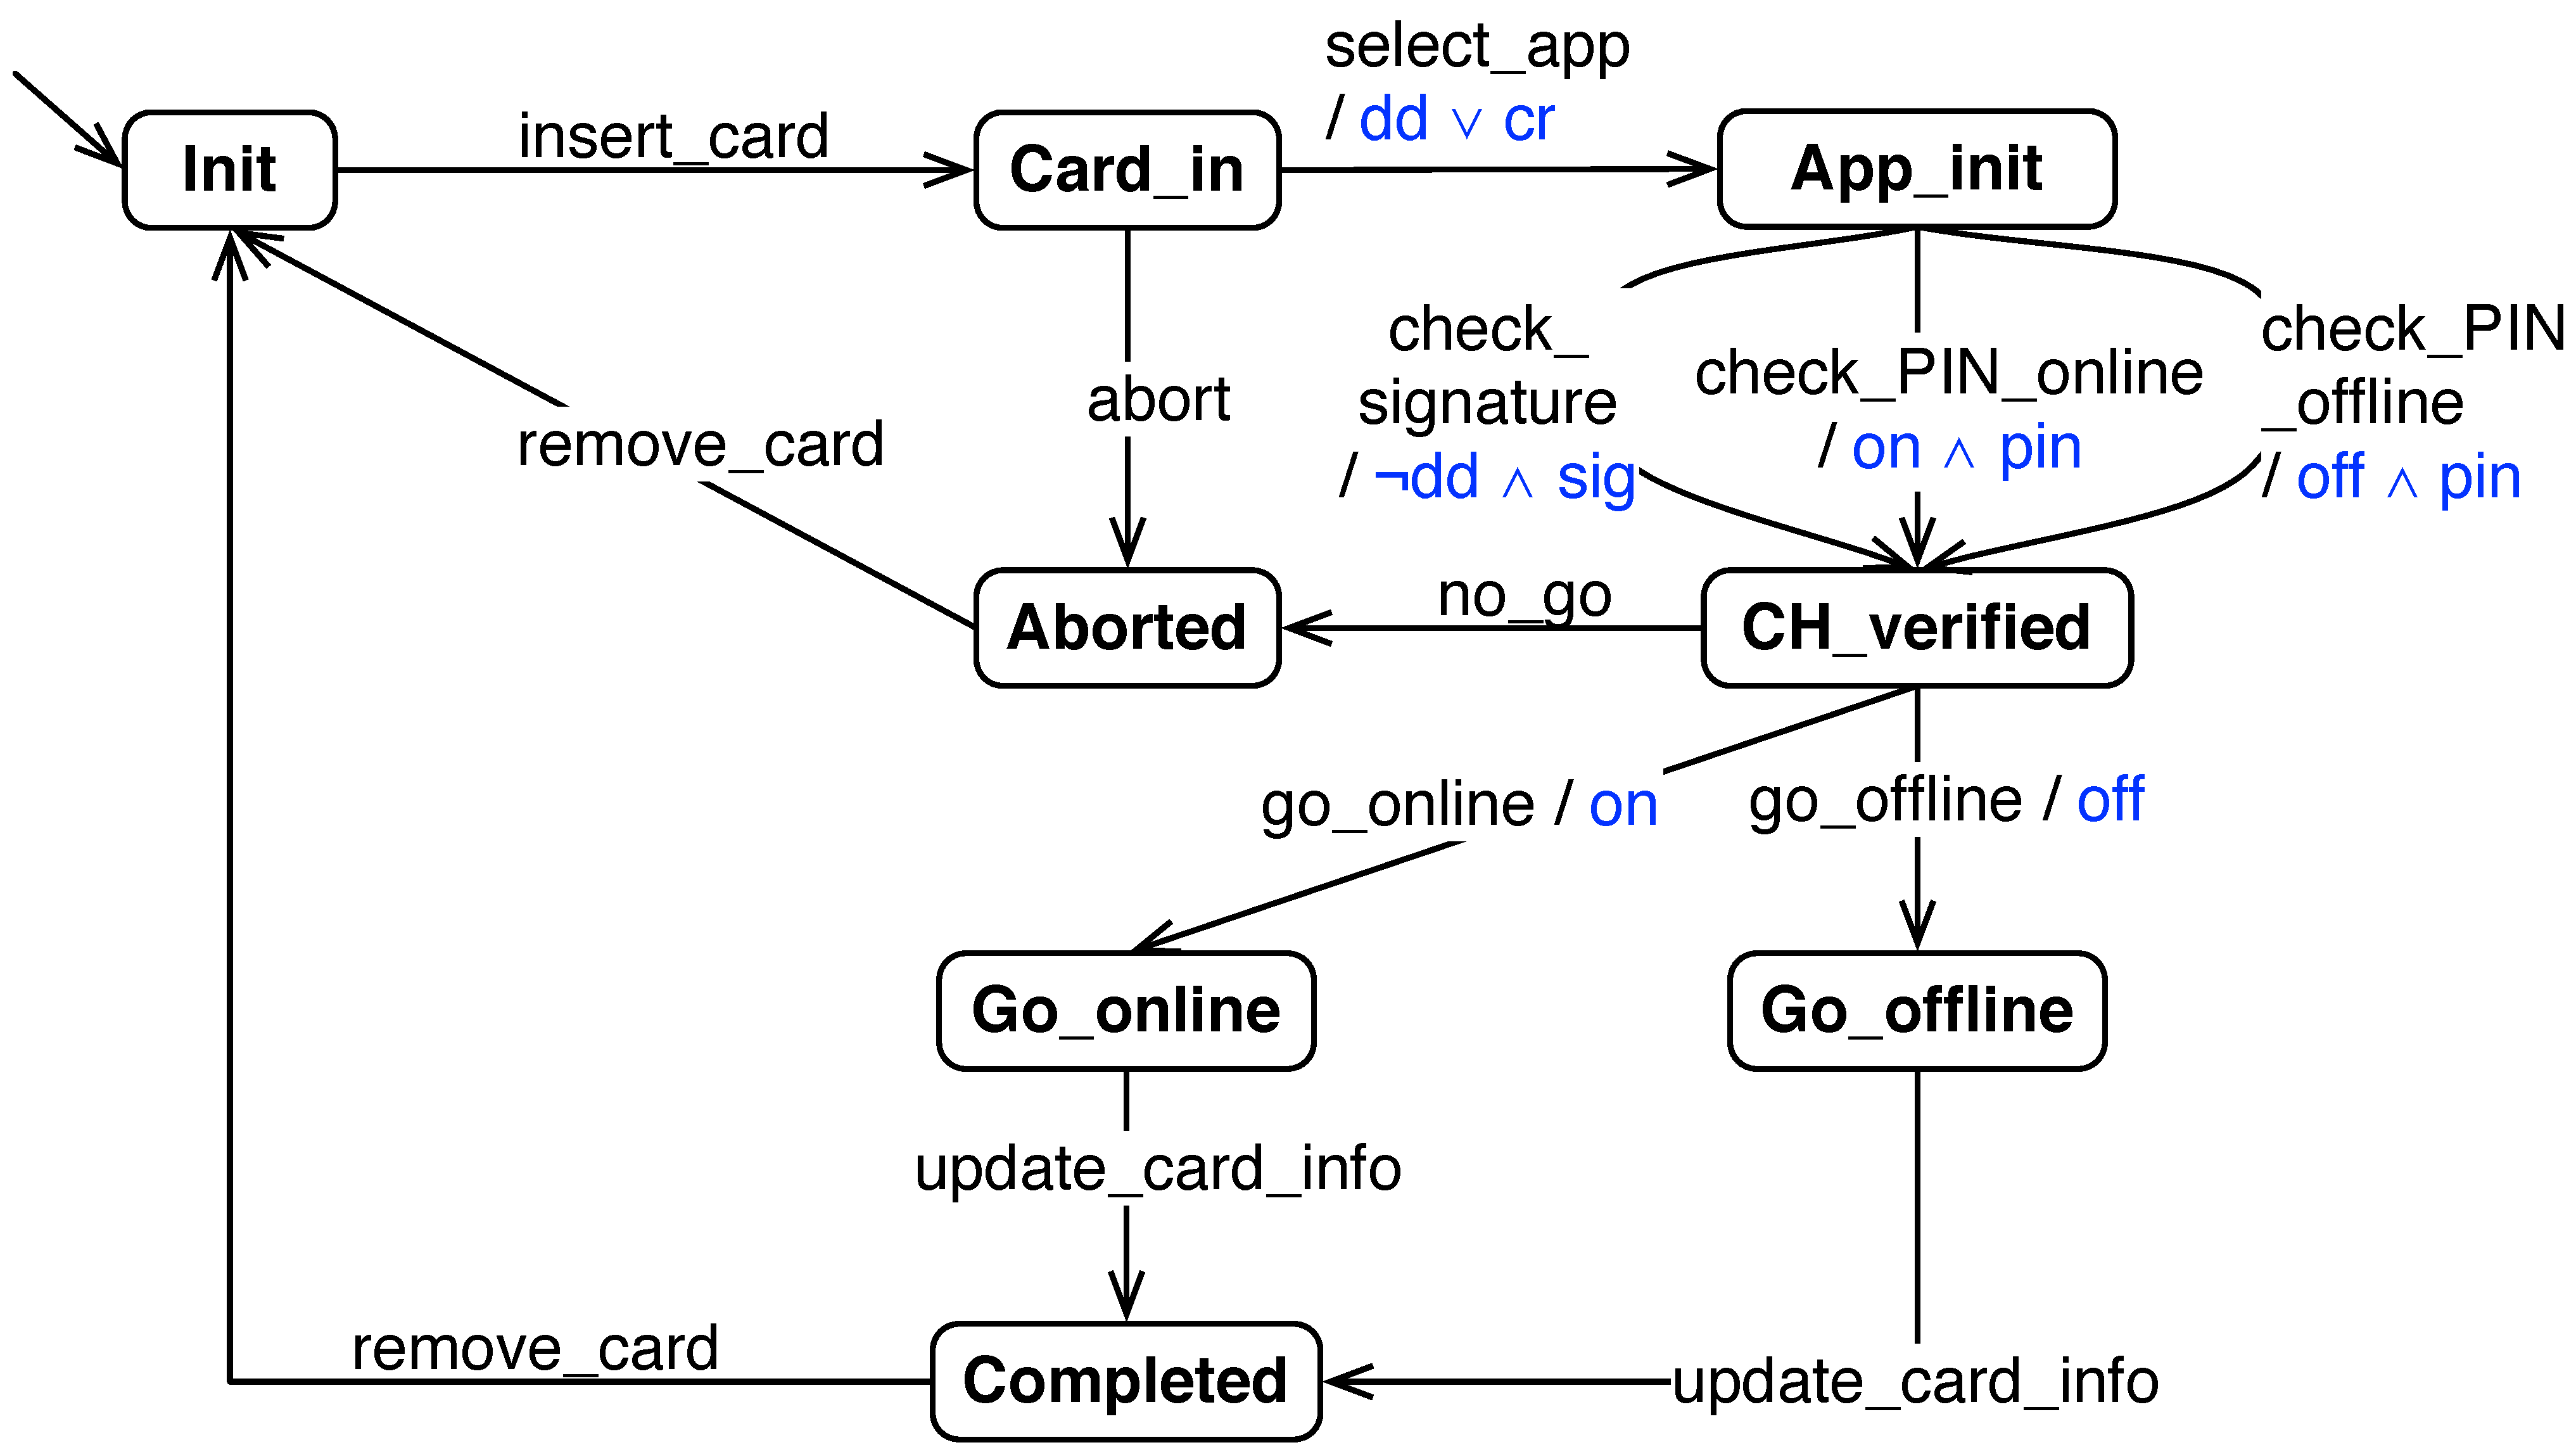
\includegraphics[width=100mm]{cpterminal-simplified-fts}
	\caption{Card payment terminal simplified \gls{featured transition system}}
	\label{fig:cpterminalsimplifiedfts}
\end{figure}

\glsreset{FTS}

Classen \etal \cite{Classen2013b} define \gls{FTS} to represent the behaviour of a product line. An \gls{FTS} is an \gls{LTS} where transitions have been annotated with feature expressions defining which products of the \gls{feature model} is able to execute the transition. For instance, the \gls{FTS} in Figure \ref{fig:cpterminalsimplifiedfts} presents the behaviour of all the products of the card payment terminal product line. The feature expressions on the transitions references the features of the feature model in Figure \ref{fig:cpterminalsimplifiedfm}. First, the terminal is initialised (\textit{Init}) and ready to proceed card payments. When a card is inserted, the terminal selects an appropriate payment method and launches the corresponding application (\textit{App\_init}). This can only be done if the terminal processes debit or credit cards, denoted by the feature expression $\mathit{dd} \vee \mathit{cr}$. Next step is to identify the card holder, either by using a \gls{PIN} code, which can be done online ($on \wedge pin$) of offline ($\mathit{off} \wedge \mathit{pin}$), or a signature if the terminal does not process debit cards ($\neg \mathit{dd} \wedge \mathit{sig}$). If the identification succeeds (\textit{CH\_Verified}), the terminal process the transaction online (\textit{Go\_online}) or offline (\textit{Go\_offline}), updates the information on the card, and completes the transaction (\textit{Completed}). Formally, \glspl{FTS} are defined as follows:
%
\begin{definition}[\acrfull{FTS} \cite{Classen2013b}]
\label{def:fts}
A \gls{FTS} is a tuple $(S,$ $\Act,$ $\trans,$ $i,$ $d,$ $\gamma)$, where:
\begin{itemize}
\item $S$, $\Act$, $\trans$, $i$ are defined according to definition \ref{def:ts}; 
\item $d$ is a \emph{feature model}; 
\item $\gamma: \trans \mapsto \Sem{d} \mapsto \mathbb{B}$  is a labelling function specifying for each transition which valid products may execute it; this function is represented as a boolean expression over the features of $d$, called \emph{\gls{feature expression}}.
\end{itemize}
\end{definition}

\begin{figure}[t]
	\centering
	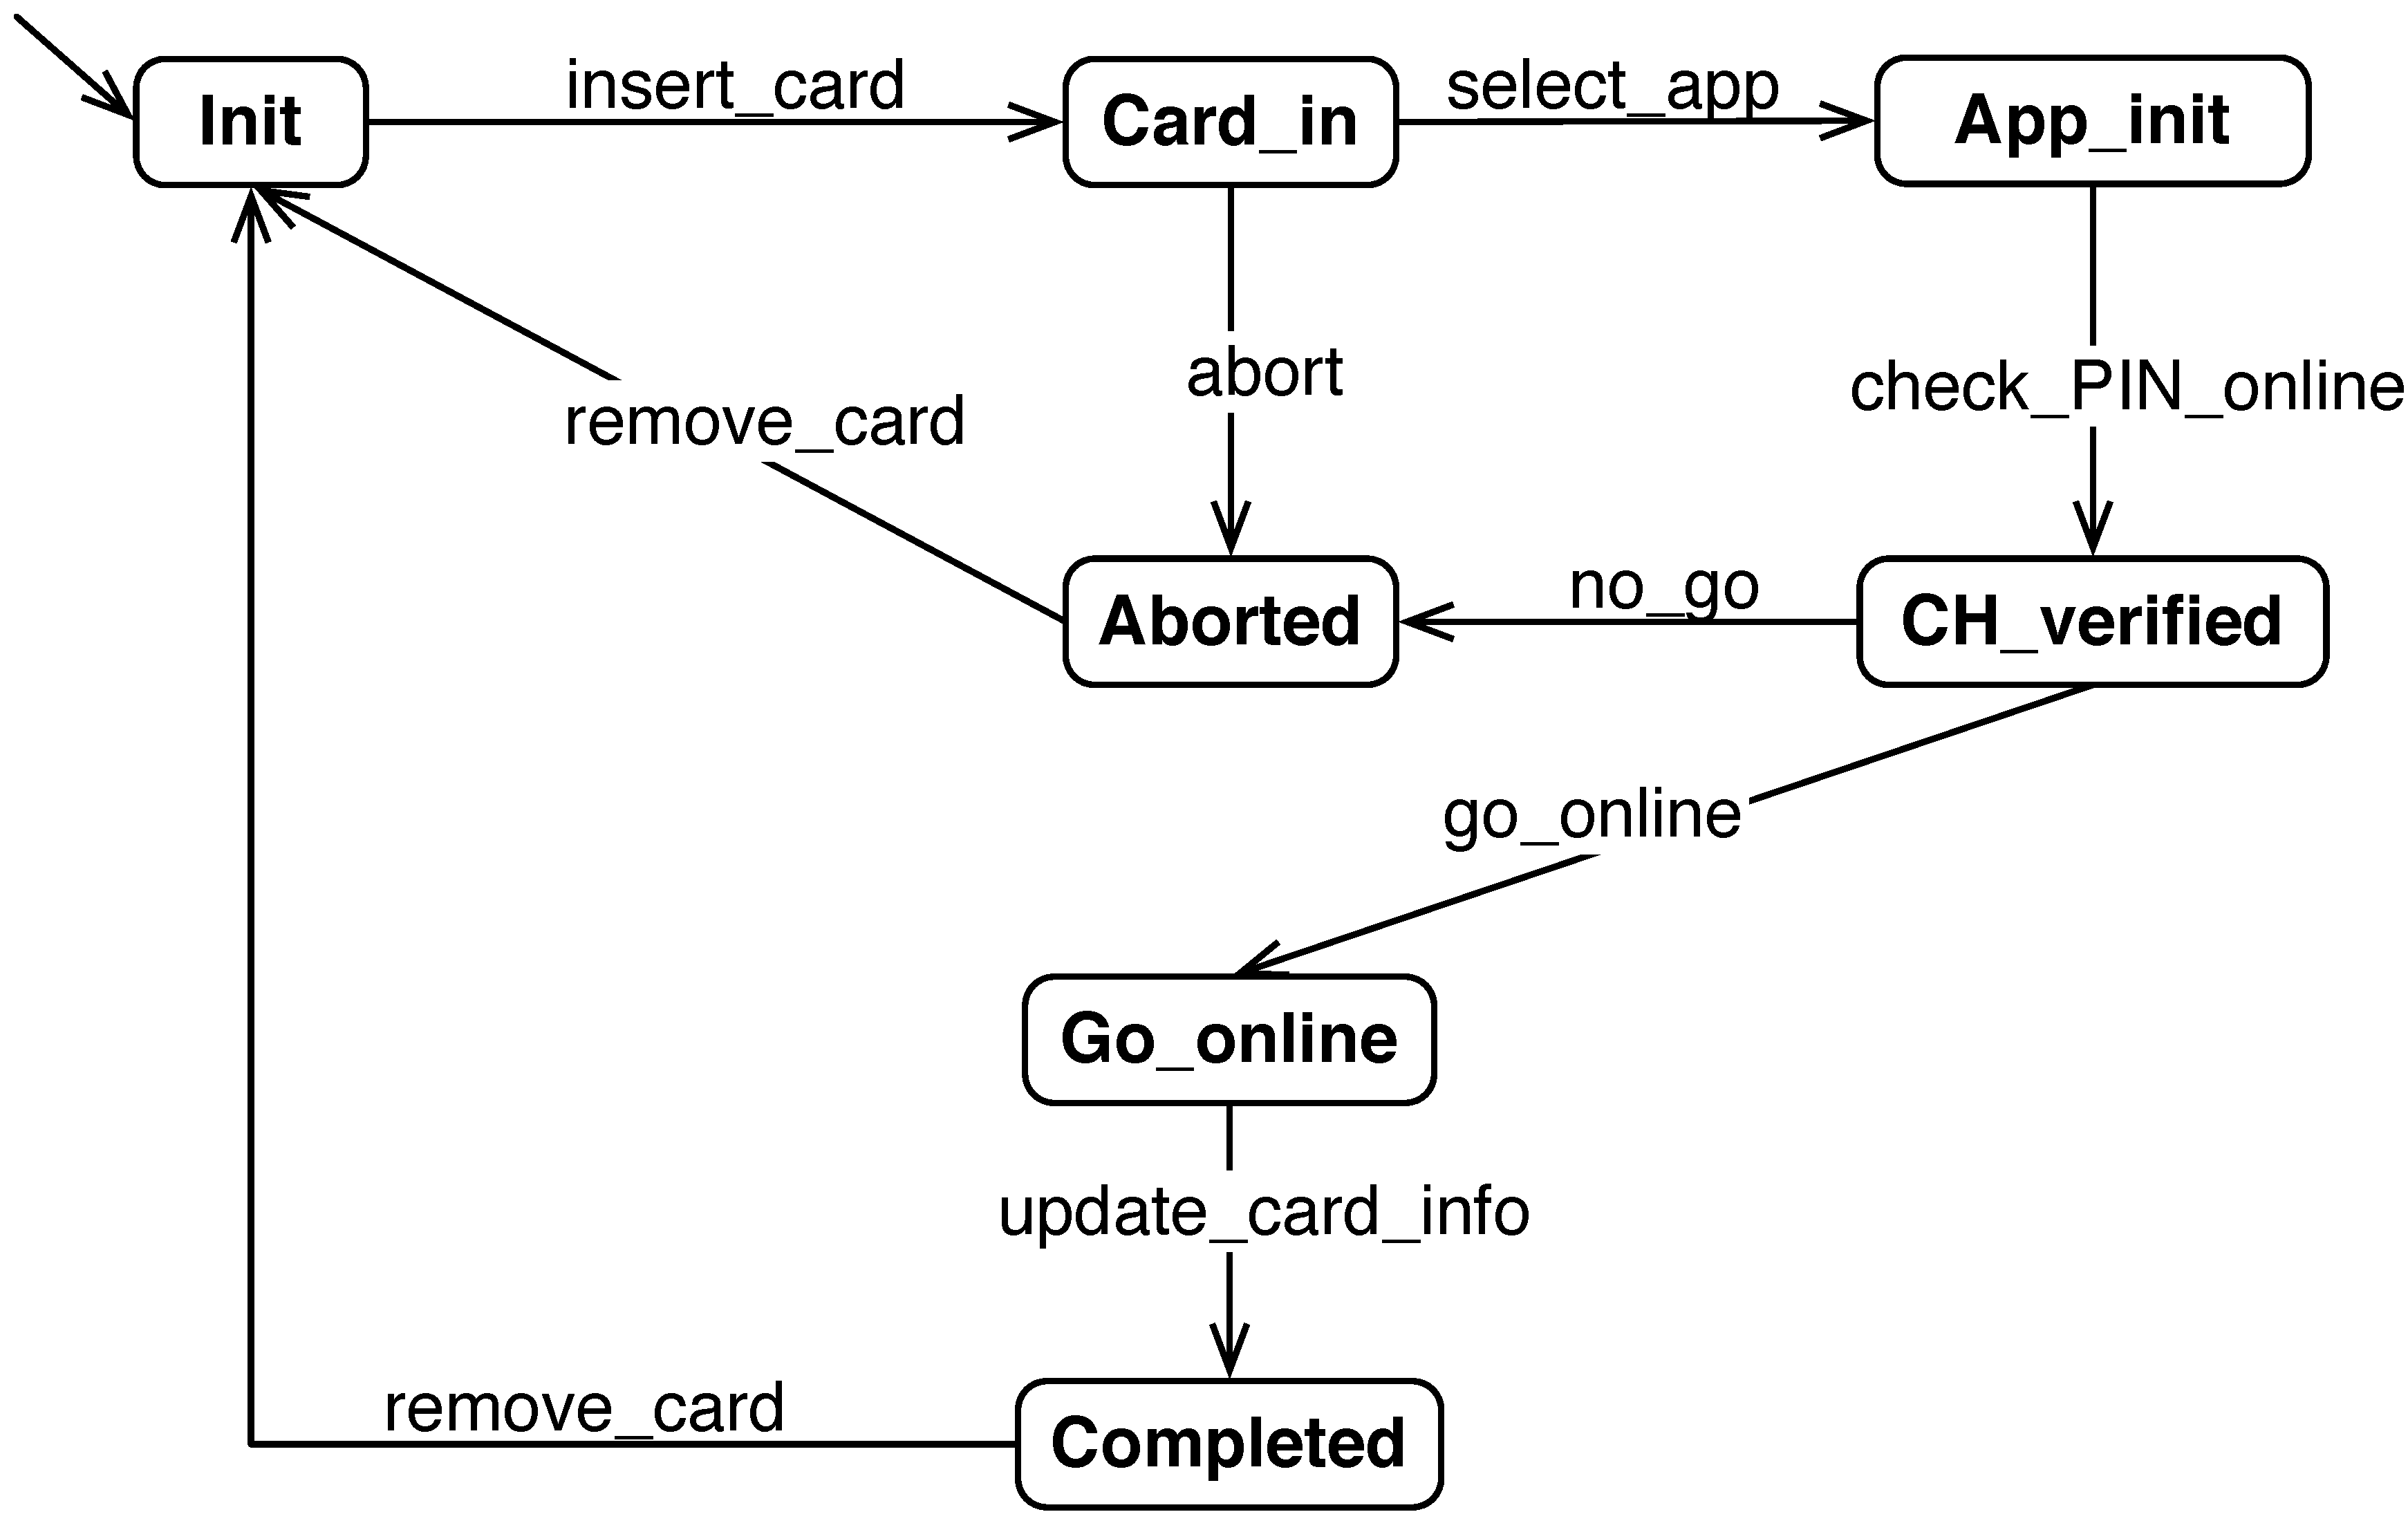
\includegraphics[width=90mm]{cpterminal-projection}
	\caption{Card payment terminal product \gls{LTS}}
	\label{fig:cpterminalprojection}
\end{figure}


\paragraph{FTS projection:}
%------------------------------

To derive the \gls{LTS} of one particular card payment terminal product, the \gls{FTS} is \emph{projected} \cite{Classen2010,Classen2013b} on this product by pruning the transitions whose feature expressions are not satisfied and by removing the feature expressions. For instance, Figure \ref{fig:cpterminalprojection} is the projection of the \gls{FTS} in Figure \ref{fig:cpterminalsimplifiedfts} on the card payment terminal product supporting direct debit (\textit{dd}) cards, with a \gls{PIN} identification (\textit{pin}) and an online connection (\textit{online}). Formally, the projection operator is defined as follows:
%
\begin{definition}[Projection operator \cite{Classen2013b}]
Let $\fts = (S,$ $\Act,$ $\trans,$ $i,$ $d,$ $\gamma)$ be an \gls{FTS}, and $p\in \Sem{d}$ be a product of the feature model $d$. The projection of $\fts$ onto $p$, denoted $\fts_{\mid p}$, is the \gls{LTS} $(S,$ $\Act,$ $\trans',$ $i)$ where
$$ \trans' = \left\lbrace \mathit{tr} \in \trans \mid \wSAT\left(p \wedge \gamma(\mathit{tr})\right) \right\rbrace $$
Where \gls{SAT} checks the satisfiability of the feature expression labelling the transition giving the product $p$.
\end{definition}


\paragraph{Deterministic FTS:}
%-----------------------------

As for \glspl{LTS}, an \gls{FTS} is deterministic if, for all sequence of actions, there is at most one possible path (sequence of transitions) for those actions. Since \gls{FTS} models the behaviour of all the products of a product line, it moreover requires to have satisfiable feature expressions on this path.
%
\begin{property}[Deterministic FTS]
An \gls{FTS} $(S,$ $\Act,$ $\trans,$ $i,$ $d,$ $\gamma)$ is deterministic if:
\begin{multline*}
\forall (\alpha_1, \ldots, \alpha_n) \in \left(\Act \cup \left\lbrace \epsilon \right\rbrace\right) ^{*},
\exists \text{ at most one } \mathit{seq} = i \xrightarrow{\alpha_1} \ldots \xrightarrow{\alpha_m} s_k \\
\text{ such that } \wSAT\left( \CNF(d) \wedge \bigwedge_{\mathit{tr} \in \mathit{seq}} \gamma(\mathit{tr}) \right)
\end{multline*}
\end{property}
%
Checking if an \gls{FTS} is deterministic is computationally heavy. In the worst case, it requires a complete exploration of the model with multiple \gls{SAT} calls.


\paragraph{Connected FTS:}
%-----------------------------

A connected \gls{FTS} is an \gls{FTS} that has no isolated state. All states may be reached from the initial state and reach back the initial state, \ie for each state, there exists a path starting from the initial state and going back to the initial state.
%
\begin{property}[Connected FTS]
An \gls{FTS} $(S,$ $\Act,$ $\trans,$ $i,$ $d,$ $\gamma)$ is connected if:
$$
\forall s \in S, \exists \mathit{seq} = i \xrightarrow{\alpha_1} \ldots \xrightarrow{\alpha_m} s \xrightarrow{\alpha_n} \ldots \xrightarrow{\alpha_o} i \text{ such that } \wSAT\left( \CNF(d) \wedge \bigwedge_{\mathit{tr} \in \mathit{seq}} \gamma(\mathit{tr}) \right)
$$
\end{property}
%
One may use (for instance) an accessibility matrix (see Algorithm \ref{algo:warshall} from Section \ref{subsec:allstatesselection}) to check that there is no isolated state. In the remainder of this thesis, most of our algorithms assume connected \glspl{FTS}.

%-------------------------------------------
\subsection{Related work}
%-------------------------------------------

We choose \gls{FTS} as formalism to model the behaviour of \glspl{SPL} over \gls{MTS} \cite{Fischbein2006} and PL-CSS \cite{Gruler2008}. \gls{MTS} is an extension of \gls{LTS} where the set of transitions is partitioned into \textit{may} and \textit{must} transitions. \textit{Must} transitions are transitions fired by all the products of the product line, while \textit{may} transitions are fired by only some (undetermined) products of the product line. To relate a transition to the exact set of products able to execute it, Asirelli \etal \cite{Asirelli2012,Asirelli2011b,Asirelli2011a} associates \gls{MTS} to a branching-time temporal logic named \gls{MHML} representing the constraints between the features and the actions. The \gls{MHML} formula may be derived from a feature model (representing those constraints) and the associated \gls{MTS} but makes the relation between products and transitions unclear.

\gls{PL-CCS} \cite{Gruler2008} is a process calculus extending Milners's \gls{CCS} \cite{Milner1982} by adding a \textit{binary variant} operator to represent alternatives features in a \gls{SPL}. As for \glspl{MTS}, PL-CSS does not include constraints between features and relies on an external \textit{mu}-calculus \cite{Shoham2012} to express them.

In their work, Beohar \etal \cite{Beohar2015} analyse the \emph{expressiveness} of \gls{FTS}, \gls{MTS}, and PL-CCS by comparing the set of products they can specify. Products specifications are represented using \glspl{LTS}. They demonstrate that \gls{FTS} is the most expressive formalism, followed by \gls{PL-CCS} and \gls{MTS}. Meaning that \gls{MTS} models may be expressed using \gls{PL-CCS}, and \gls{PL-CCS} models may be expressed using \gls{FTS} but not (always) the other way around.


%%%%%%%%%%%%%%%%%%%%%%
\section{Wrap up}
%%%%%%%%%%%%%%%%%%%%%%

In this chapter, we presented the standard software product line engineering process and focuses on domain level to perform behavioural model-based testing, \ie selecting relevant products and behaviour to test in the product line. \gls{SPL} variability is encoded using a boolean \gls{feature model} and behaviour is described using an annotation-based formalism: a connected \gls{FTS}. We choose \glspl{FTS} for their expressiveness and the simplicity of their encoding allowing powerful algorithms \cite{Classen2013b,Cordy2013} while preserving a readable relation between transitions and products able to execute them.

